\chapter{图像处理模块}
YOLOv8建立在以前YOLO版本的成功基础上, 引入了新的功能和改进,进一步提高了性能和灵活性。YOLOv8设计快速、准确且易于使用,是目标检测和跟踪、实例分割、图像分类和姿态估计任务的绝佳选择。并且代码开发完善,适合快速开发和部署。从训练到部署的完整流程可参考\href{https://doc.embedfire.com/linux/rk356x/Ai/zh/latest/lubancat_ai/example/yolov8.html}{鲁班猫AI开发指南}。
\section{yolov8环境配置}
在个人PC上使用conda创建虚拟环境,安装\href{https://github.com/ultralytics/ultralytics}{ultralytics}相关环境。
\section{模型训练}

\subsection{数据集处理}
使用anylabeling工具对数据集进行标注,生成YOLO格式的标签文件。以下是处理步骤:
\begin{enumerate}
    \item 使用anylabeling工具打开数据集目录。
    \item 选择需要标注的图像,进行标注操作(可以通过AI模型辅助标注)。
    \item 导出标注结果为YOLO格式,保存到指定目录。
\end{enumerate}
\subsection{yolov8-seg模型训练}
使用YOLOv8-seg模型进行图像分割训练,以下是训练方法:
\begin{lstlisting}[language=bash, basicstyle=\ttfamily\small, keywordstyle=\color{blue}, breaklines=true]
yolo segment train model=yolov8n-seg.pt data=coco128-seg.yaml epochs=100 imgsz=640
\end{lstlisting}
其中,`coco128-seg.yaml`是数据集配置文件,包含类别信息和训练集、验证集路径。`yolov8n-seg.pt`是预训练模型,可以根据需要选择其他版本的YOLOv8模型。
简单评估:
\begin{lstlisting}[language=bash, basicstyle=\ttfamily\small, keywordstyle=\color{blue}, breaklines=true]
yolo segment val model=runs/segment/train/best.pt
\end{lstlisting}
\subsection{训练结果}
训练结果:
\begin{figure}[H]  % "h!" 表示尽可能在当前位置插入
    \centering  % 图片居中
    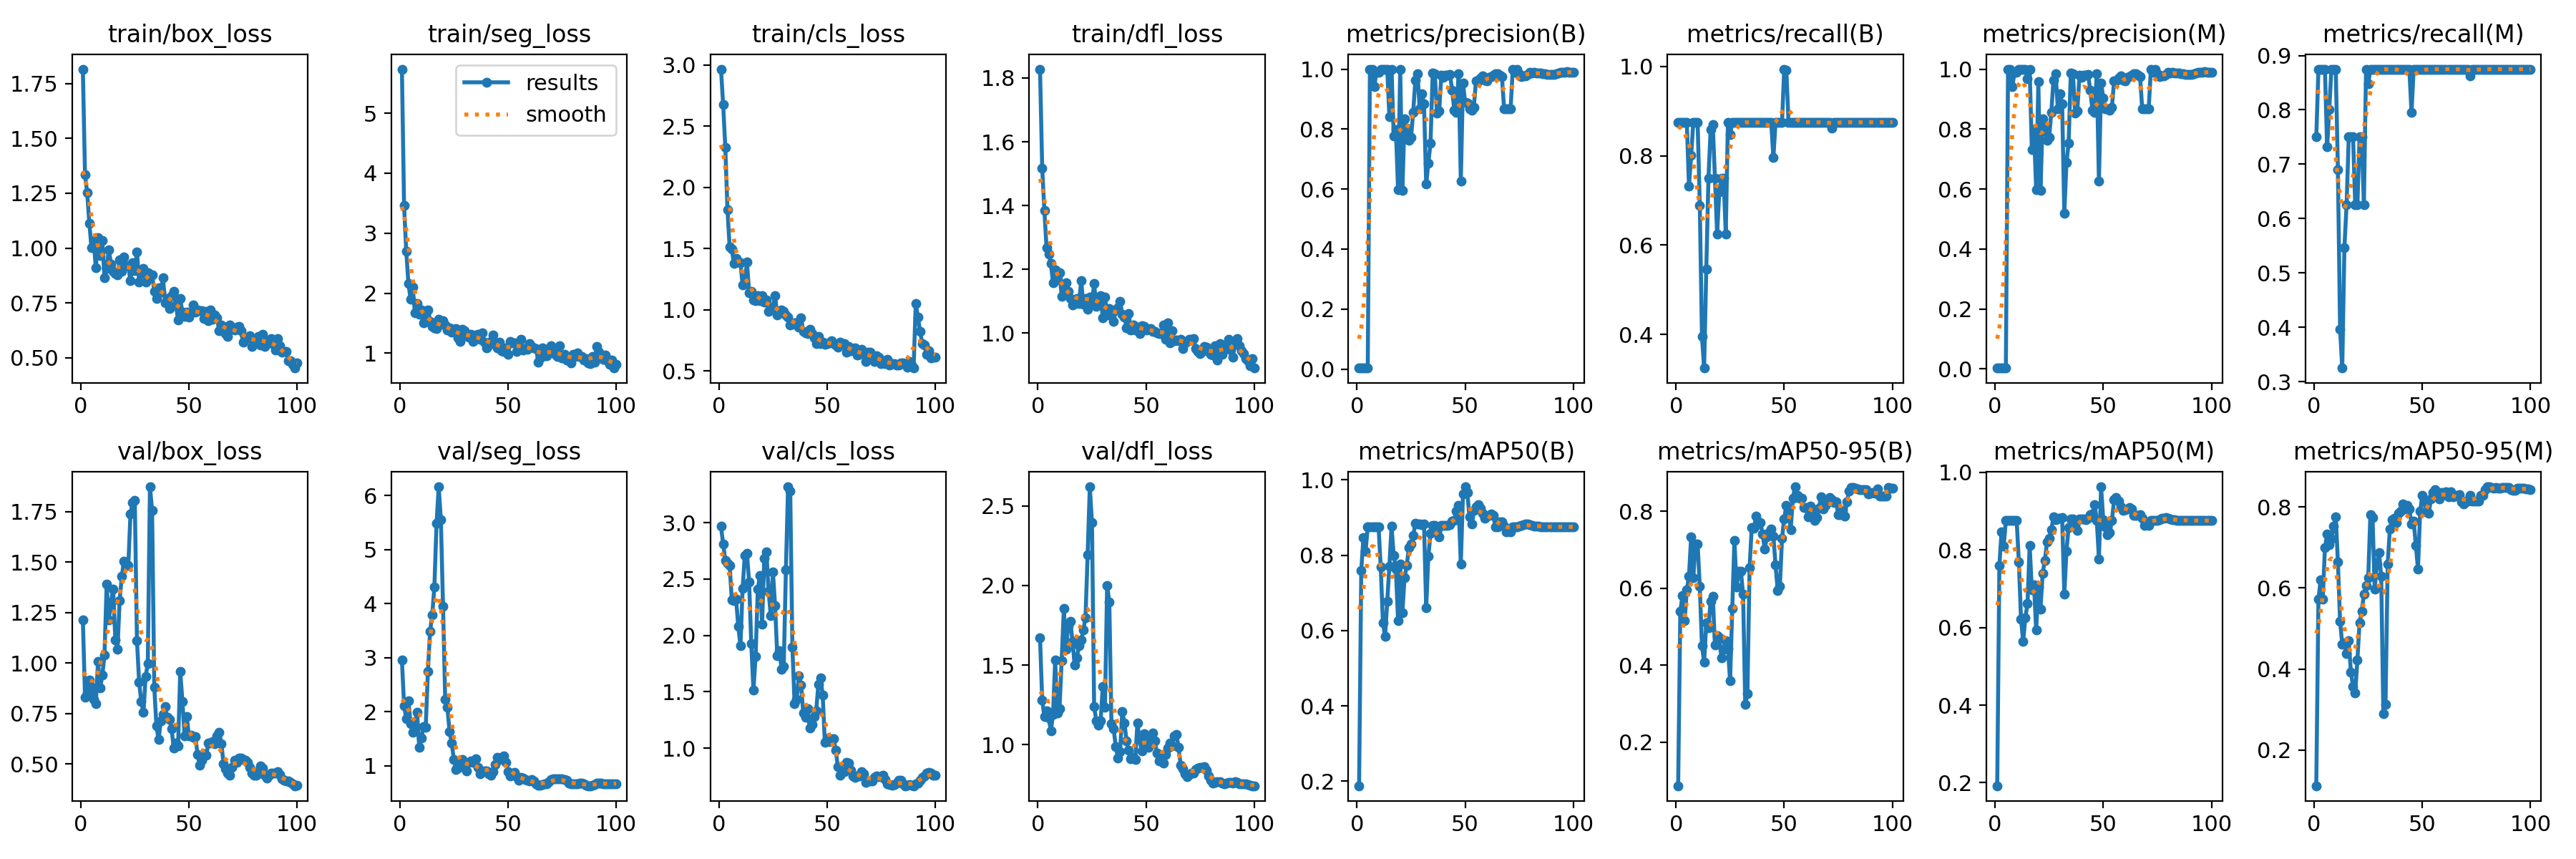
\includegraphics[width=1.0\textwidth]{results.png}  % 图片文件路径,设置宽度为页面宽度的80%
    \caption{整体训练结果。}  % 图片标题
\end{figure}
\begin{figure}[H]  % "h!" 表示尽可能在当前位置插入
    \centering  % 图片居中
    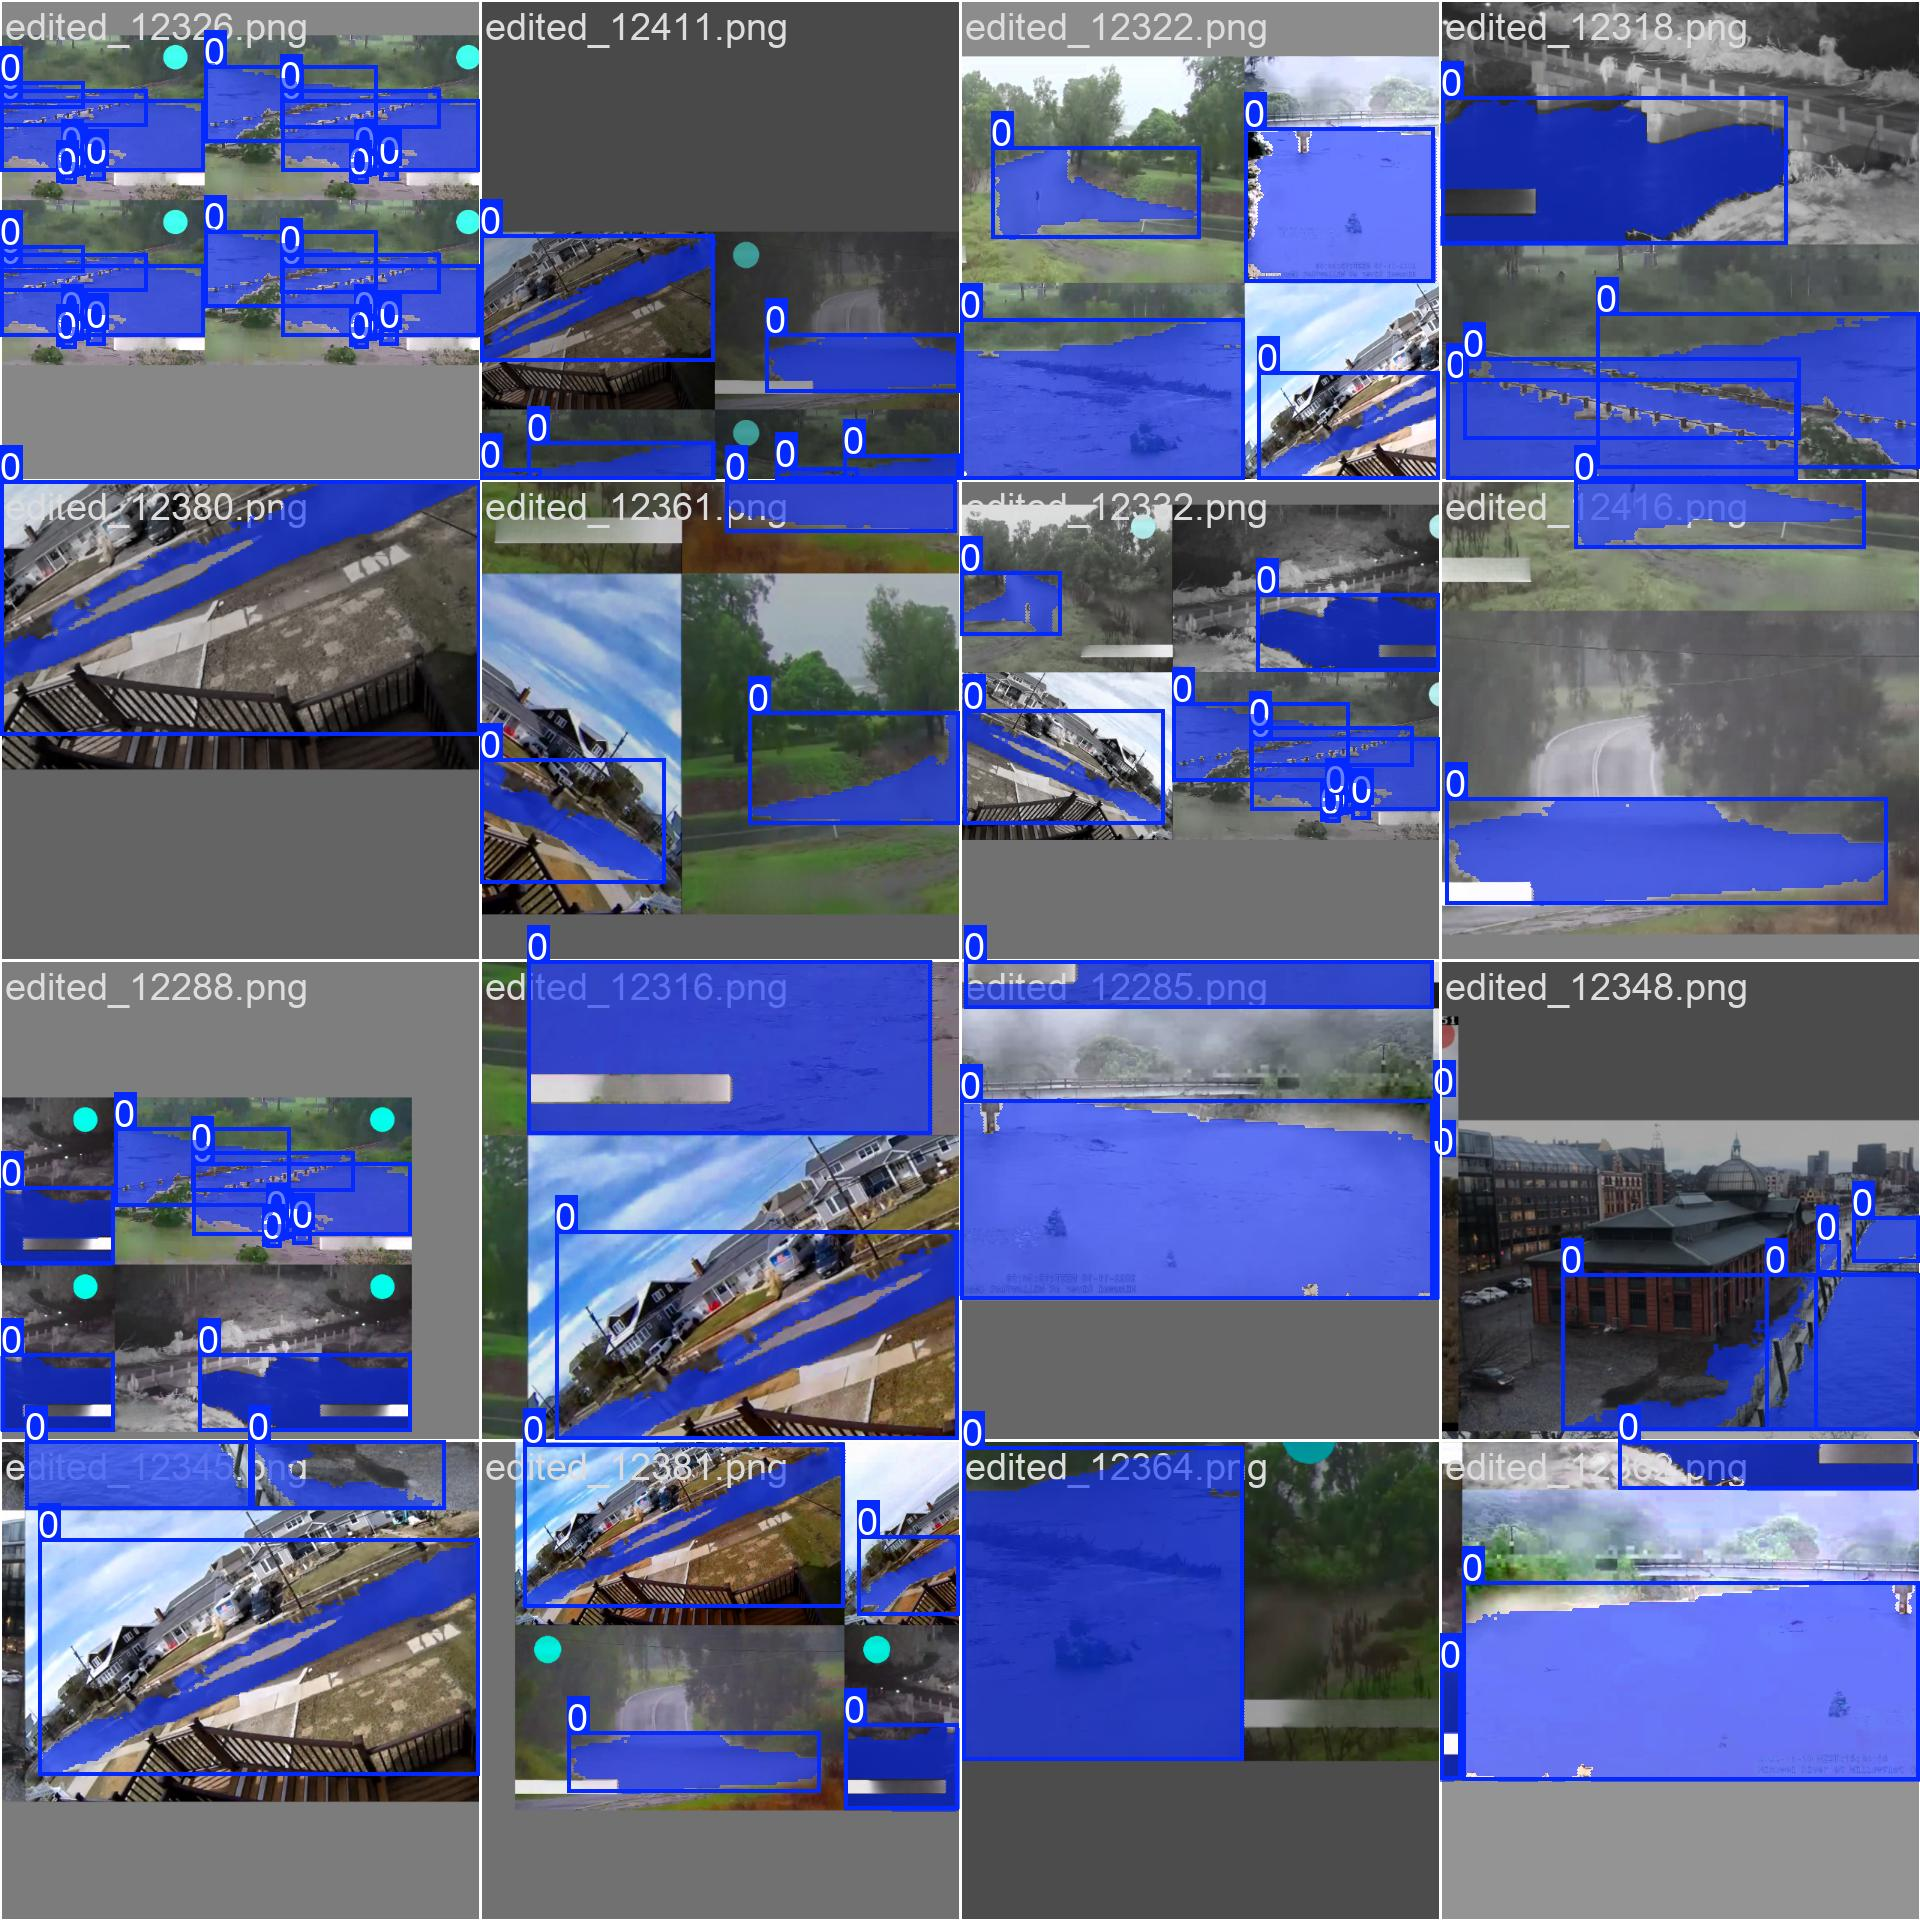
\includegraphics[width=1.0\textwidth]{train_batch0.jpg}  % 图片文件路径,设置宽度为页面宽度的80%
    \caption{部分训练集。}  % 图片标题
\end{figure}
\begin{figure}[H]  % "h!" 表示尽可能在当前位置插入
    \centering  % 图片居中
    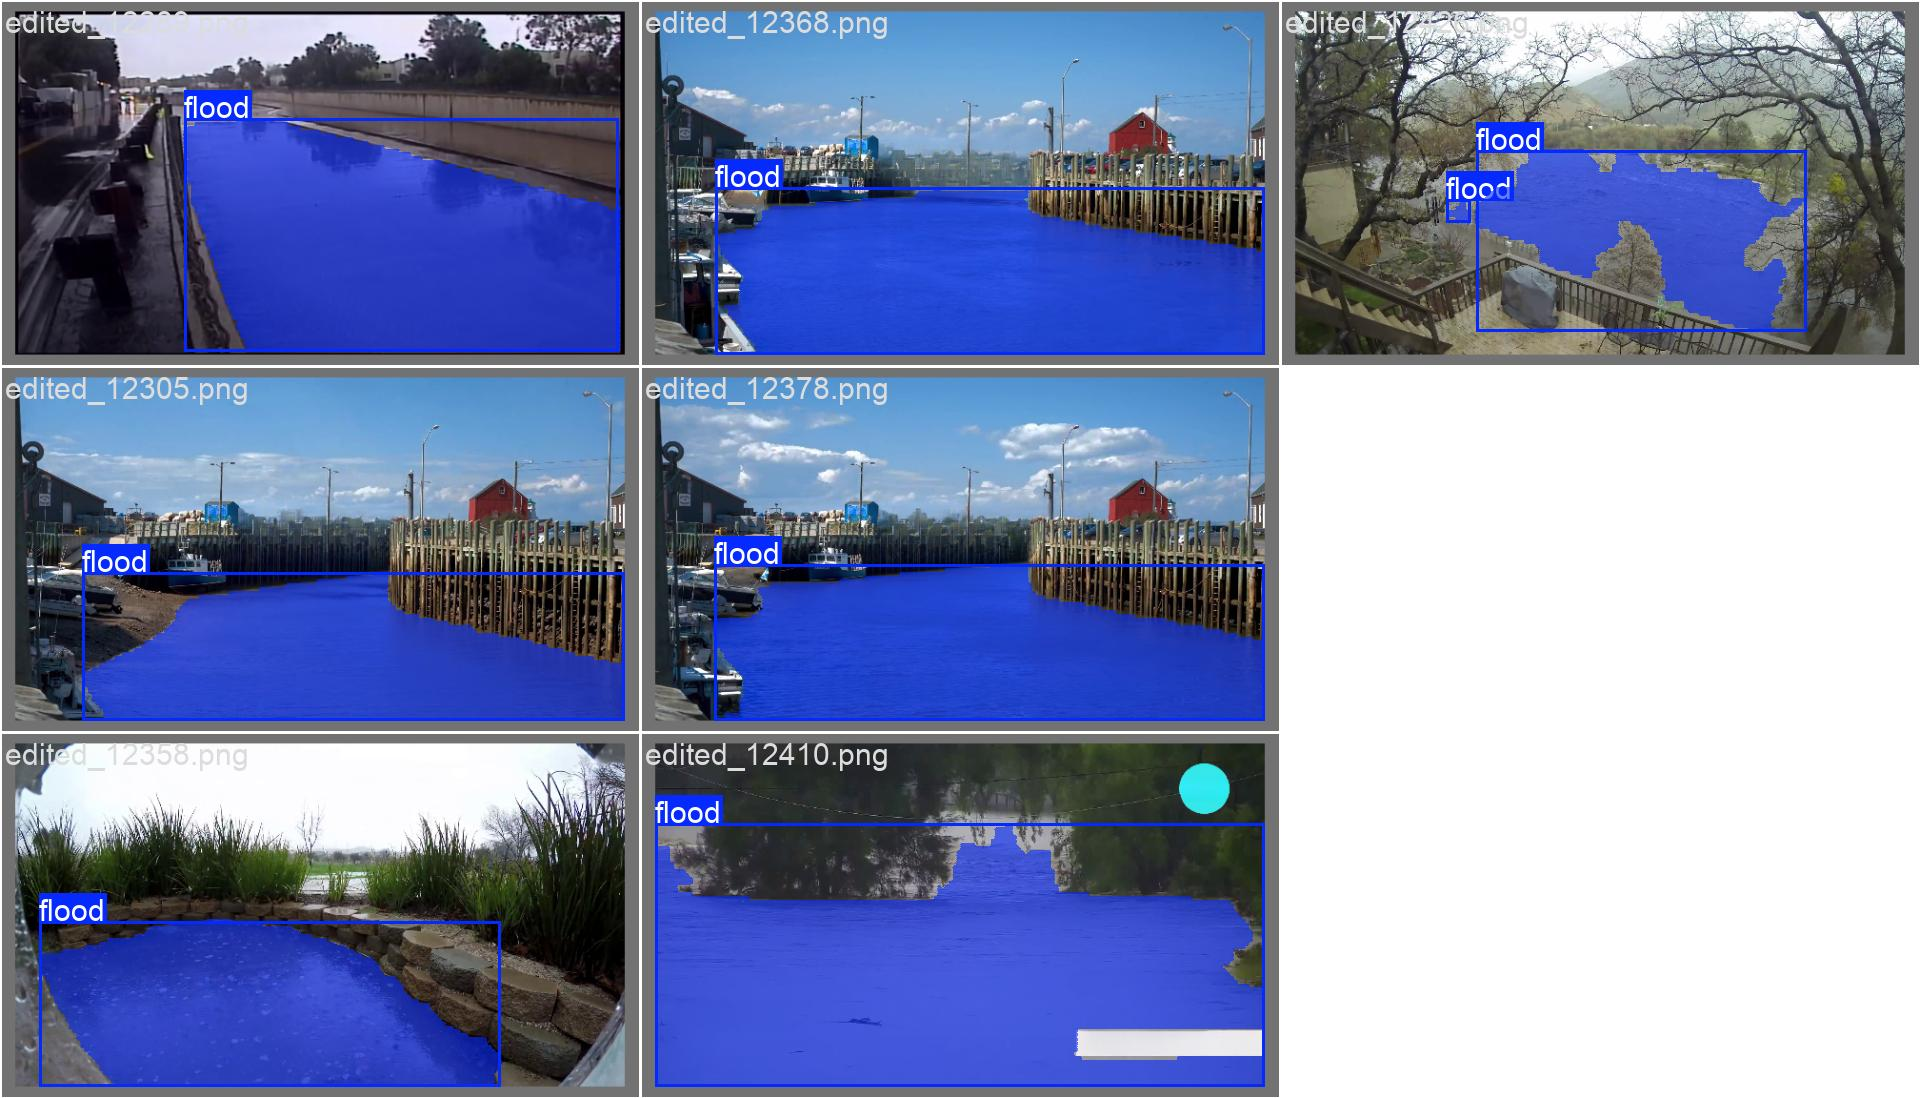
\includegraphics[width=1.0\textwidth]{val_batch0_labels.jpg}  % 图片文件路径,设置宽度为页面宽度的80%
    \caption{验证集。}  % 图片标题
\end{figure}
\begin{figure}[H]  % "h!" 表示尽可能在当前位置插入
    \centering  % 图片居中
    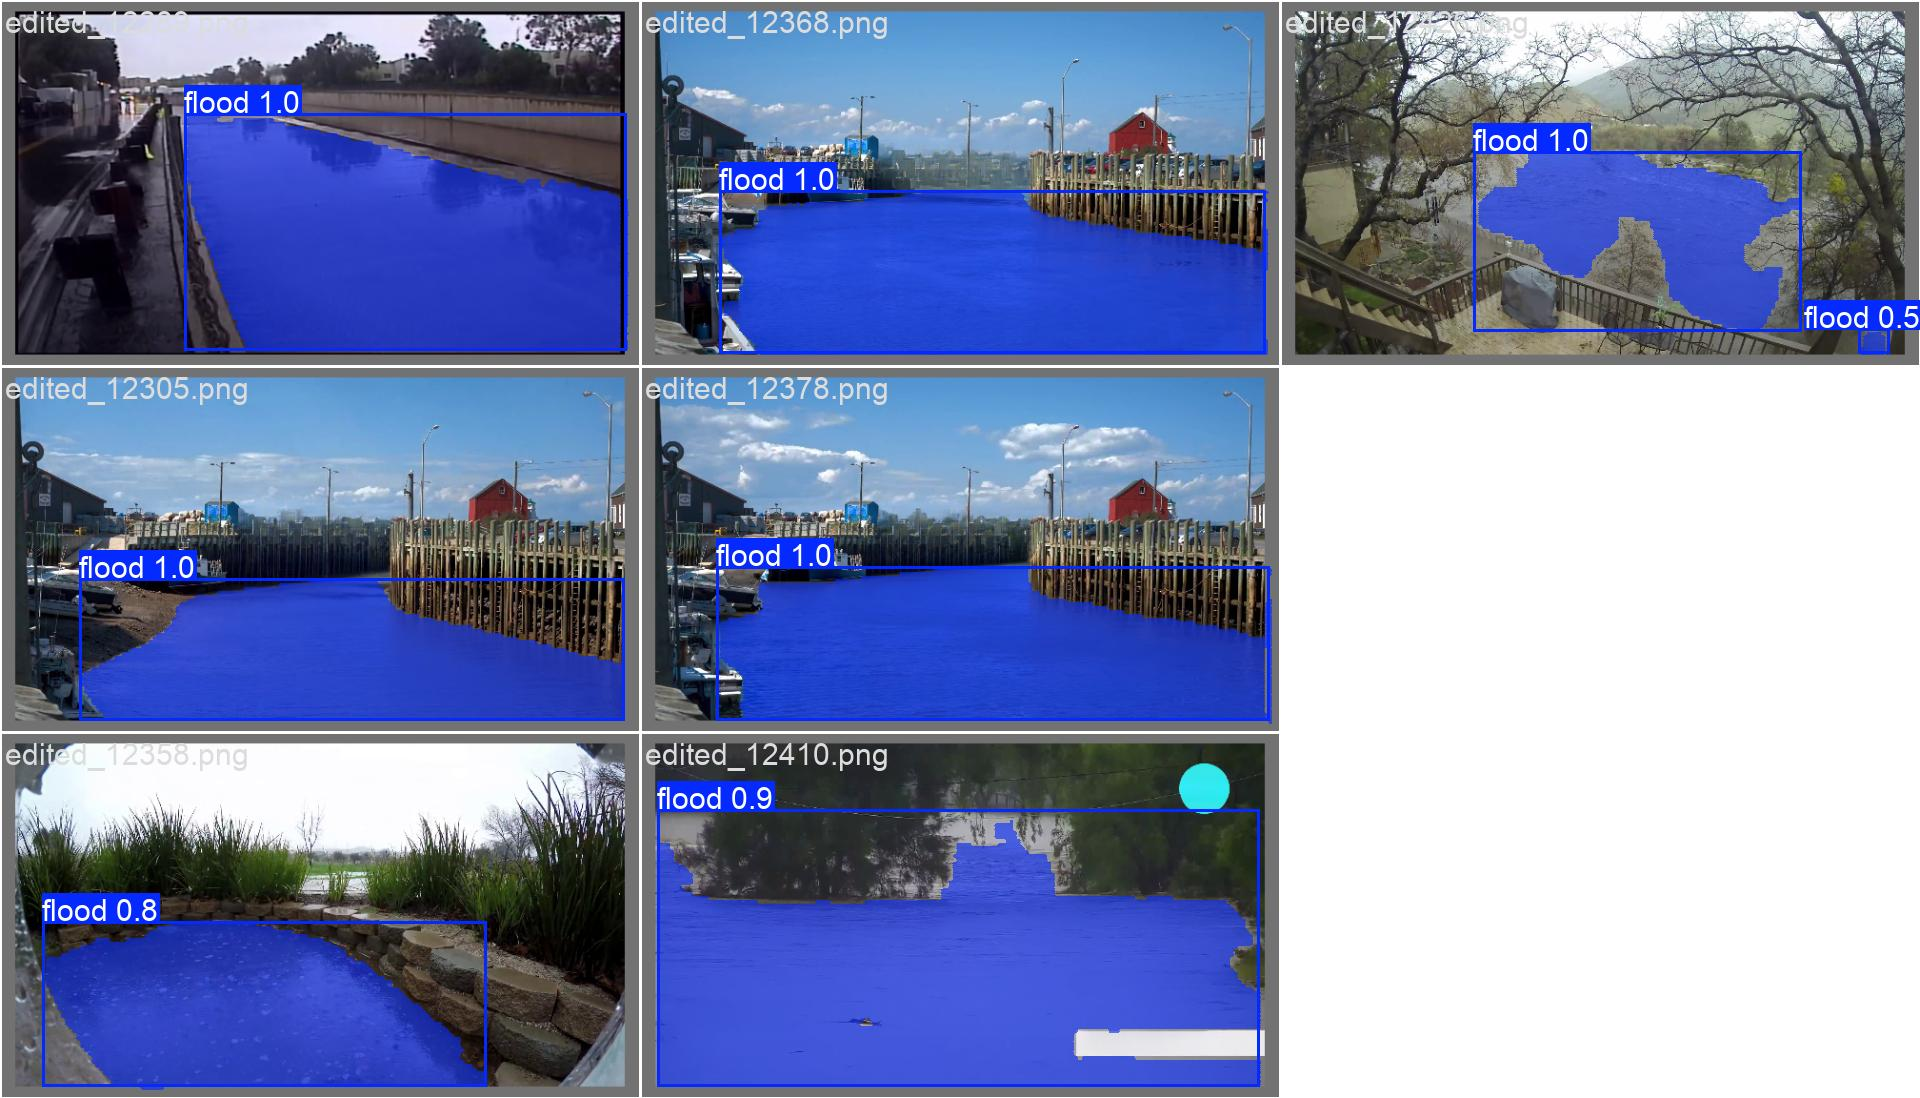
\includegraphics[width=1.0\textwidth]{val_batch0_pred.jpg}  % 图片文件路径,设置宽度为页面宽度的80%
    \caption{验证结果。}  % 图片标题
\end{figure}
\section{模型导出}
使用\href{https://github.com/airockchip/ultralytics_yolov8}{ultralytics}提供的export方法导出适合部署到rknpu上的模型,该模型在npu上获得更高的推理效率。

\section{模型转换}
导出的模型,还需要通过toolkit2转换成rknn模型,可参考\href{https://github.com/airockchip/rknn_model_zoo/tree/main/examples/yolov8}{rknn\_model\_zoo仓库的例程}。编译模型转换程序,转换成rknn模型。(需要在linux系统中转换,不支持Windows系统)
\section{模型部署}
\noindent 下载\href{https://gitee.com/LubanCat/lubancat_ai_manual_code.git}{配套例程}将转换好rknn模型放到model目录下:
\begin{lstlisting}[language=bash, basicstyle=\ttfamily\small, keywordstyle=\color{blue}]
/home/cat/lubancat_ai_manual_code/example/yolov8/yolov8_seg/model
同时需要修改model目录中coco_80_labels_list.txt的类别的数量和名称
\end{lstlisting}
切换到模型路径:
\begin{lstlisting}[language=bash, basicstyle=\ttfamily\small, keywordstyle=\color{blue}]
cd lubancat_ai_manual_code/example/yolov8/yolov8_det/cpp
\end{lstlisting}
编译模型:
\begin{lstlisting}[language=bash, basicstyle=\ttfamily\small, keywordstyle=\color{blue}]
 ./build-linux.sh -t rk3588
\end{lstlisting}
这里rk3588是鲁班猫4的芯片型号。
编译完成后,生成的可执行文件 `rknn\_yolov8\_demo` 在当前目录下的 \texttt{install/rk3588\_linux} 目录下。
模型运行:
\begin{lstlisting}[language=bash, basicstyle=\ttfamily\small, keywordstyle=\color{blue}]
./rknn_yolov8_demo ./model/yolov8_rk3588.rknn ./model/1.jpg
\end{lstlisting}
运行结果如下图所示:
\begin{figure}[h!]  % "h!" 表示尽可能在当前位置插入
    \centering  % 图片居中
    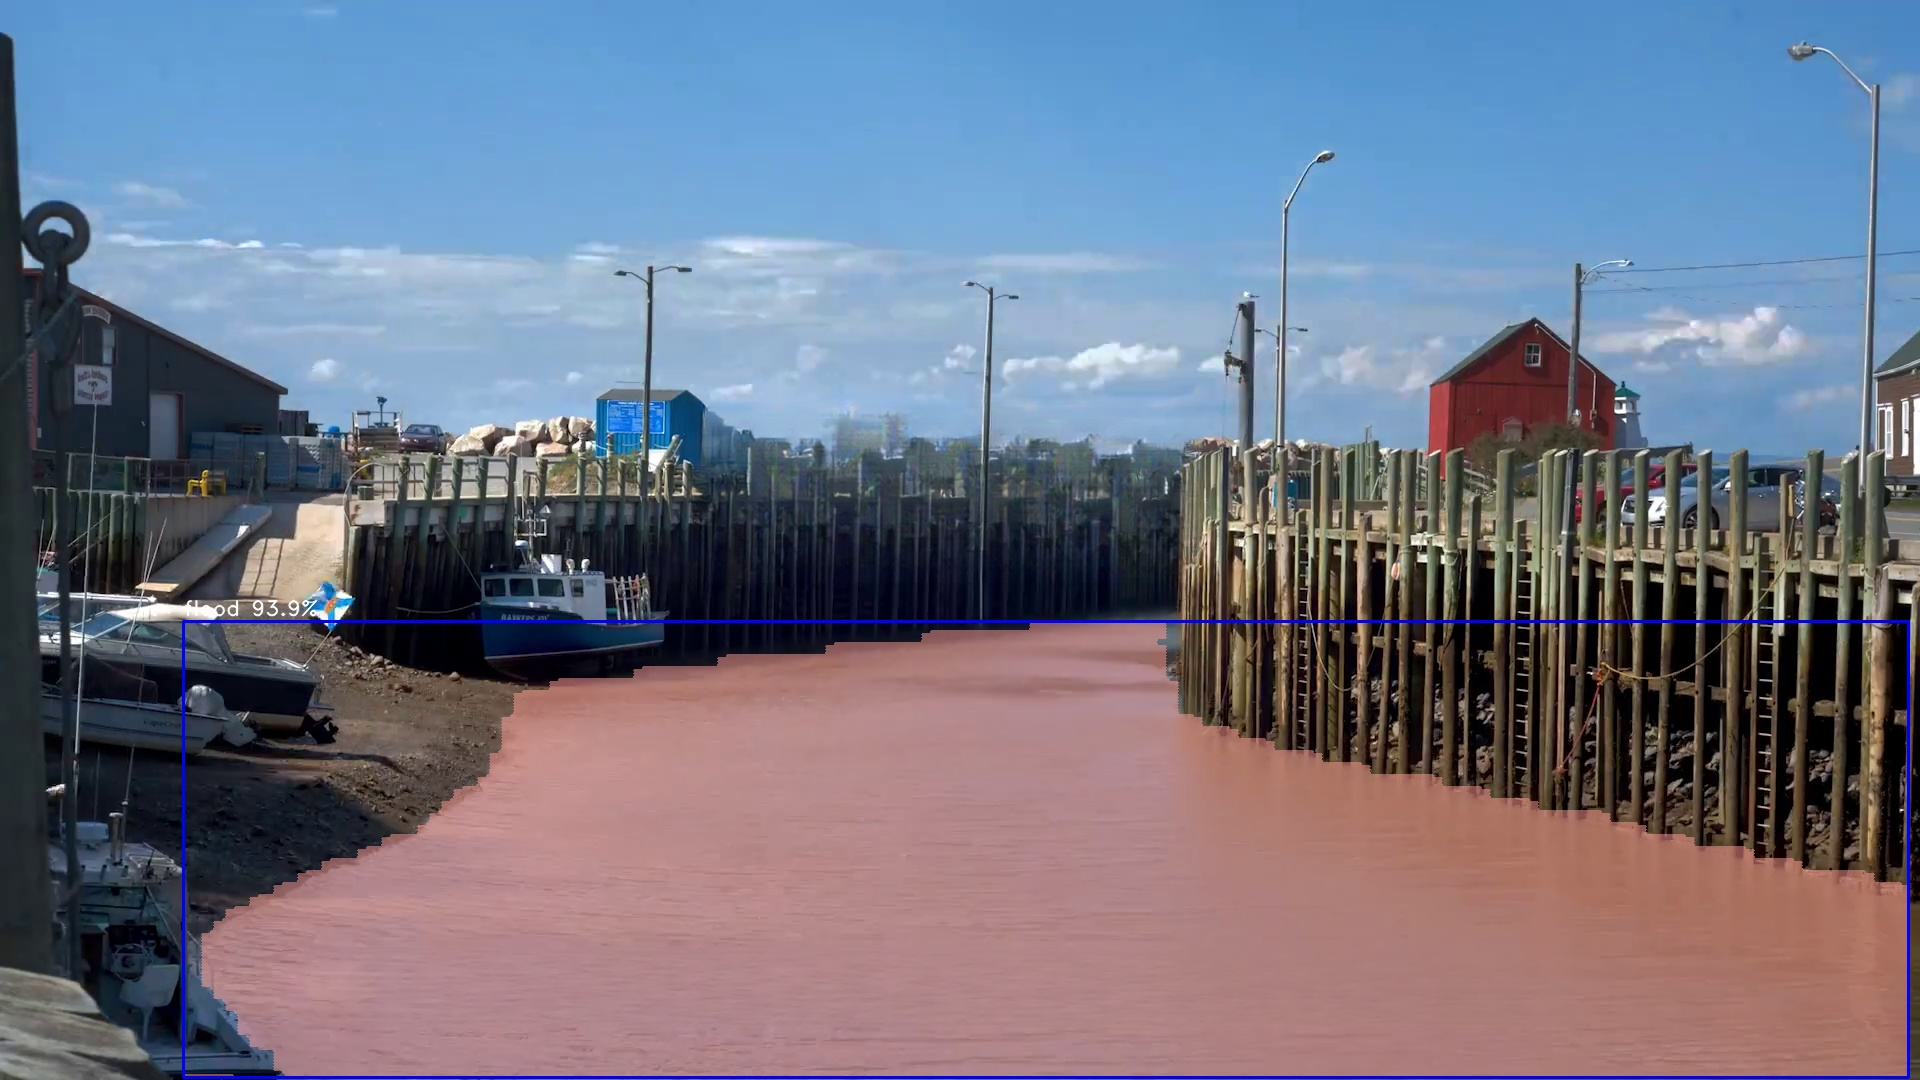
\includegraphics[width=1.0\textwidth]{out.jpg}  % 图片文件路径,设置宽度为页面宽度的80%
    \caption{鲁班猫的模型识别结果。}  % 图片标题
\end{figure}

\section{Rust服务器集成yolov8-seg推理模型}
本项目服务器端采用Rust语言实现,负责接收前端请求、采集摄像头图片,并调用yolov8-seg C++推理模型进行分割推理,最后将推理结果图片返回给前端。由于yolov8推理模型为C++可执行文件,需在Rust服务器中实现跨语言调用与结果处理。
\subsection{图片采集与保存}
服务器通过OpenCV采集摄像头图片,并将图片以唯一id命名保存到指定路径。例如:
\begin{lstlisting}[language=bash, breaklines=true]
let image_path = format!("/path/to/images/{}.jpg", image_id);
// 使用 OpenCV 采集并保存图片到 image_path
\end{lstlisting}
\subsection{配置yolov8推理可执行文件}
\begin{itemize}
    \item yolov8 C++推理可执行文件路径:\\
    \lstinline[breaklines=true]|/home/cat/lubancat_ai_manual_code/example/yolov8/yolov8_seg/cpp/install/rk3588_linux/rknn_yolov8_seg_demo|
    \item 模型文件路径:\\
    \lstinline[breaklines=true]|/home/cat/lubancat_ai_manual_code/example/yolov8/yolov8_seg/cpp/install/rk3588_linux/model/yolov8n-seg.rknn|
\end{itemize}
\subsection{Rust中调用C++可执行文件}
Rust使用\texttt{std::process::Command}调用外部C++推理程序,传递模型路径和图片路径作为参数:
\begin{lstlisting}[language=Rust]
use std::process::Command;

let output = Command::new(exe_path)
    .arg(model_path)
    .arg(&image_path)
    .output()
    .expect("failed to execute yolov8 seg demo");

if !output.status.success() {
    // 错误处理
}
\end{lstlisting}

\subsection{读取推理结果}

C++推理程序完成后,将推理结果图片保存到指定路径。随后,将推理图片传输至服务端,服务端来读取图片内容。
\subsection{HTTP路由集成}

在Actix-web框架下,新增\texttt{/yolov8/\{id\}}路由,处理前端推理请求:

\begin{lstlisting}[language=bash, breaklines=true]
#[get("/yolov8/{id}")]
pub async fn yolov8_infer(
    id: web::Path<u32>,
) -> actix_web::Result<HttpResponse> {
    let id = id.into_inner();
    let image_path = format!("/path/to/images/{}.jpg", id);

    // ...调用 C++ 推理和读取图片...

    Ok(HttpResponse::Ok()
        .content_type("image/jpeg")
        .body(img_bytes))
}
\end{lstlisting}

\subsection{路由注册}

在\texttt{main.rs}中注册yolov8路由:

\begin{lstlisting}[language=Rust]
App::new()
    .service(api::yolov8_infer)
\end{lstlisting}

\subsection{测试方法}

\begin{enumerate}
    \item 启动Rust服务器:
    \begin{lstlisting}[language=bash]
cargo run
    \end{lstlisting}
    \item 通过curl或浏览器访问接口,例如:
    \begin{lstlisting}[language=bash]
curl -o result.jpg http://localhost:8080/yolov8/1
    \end{lstlisting}
    \item 检查返回图片是否为推理结果。
\end{enumerate}

\section{模型可扩展性}

本节介绍图像分割与检测模型在不同应用场景下的扩展方法,包括灾难识别、跌倒检测等,并探讨多种可实现的技术路线和优化建议。

\subsection{灾难识别}

对于不同类型的灾难(如泥石流、火灾、洪水等),只需准备相应的灾难场景数据集,并对感兴趣的区域进行标注,即可沿用本章介绍的完整流程(数据标注、模型训练、模型导出与部署)进行模型开发。若需实现多灾难联合识别,可在同一数据集中为不同灾难类型分别标注区域,训练时将类别数设置为灾难类型总数。训练完成后,模型即可在一张图片中同时识别出多种灾难区域。

提升识别精度的方法包括:
\begin{itemize}
    \item 选用更高性能的模型,如YOLOv8的更大版本(yolov8x-seg 等)或最新的YOLO系列(如 YOLOv11)。
    \item 尝试使用更先进的分割模型,如Segment Anything Model(SAM)或SAM2。需要注意,虽然 SAM2 等模型精度更高,但参数量和计算量也显著增加。例如,SAM2 的参数量约为 yolov8n-seg 的11倍,且在CPU上的推理速度慢1000倍以上,实际部署时需权衡精度与速度,如图\ref{fig:yolo_sam}所示。
\end{itemize}
\begin{figure}[H]  % "h!" 表示尽可能在当前位置插入
    \centering  % 图片居中
    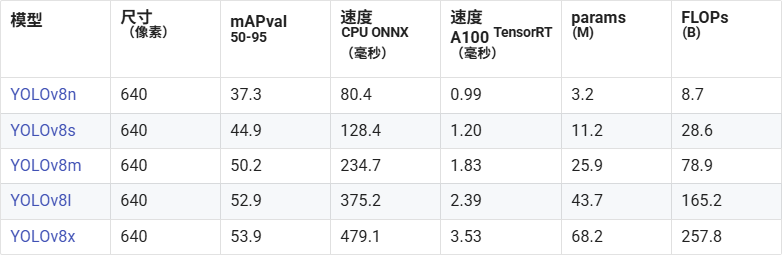
\includegraphics[width=1.0\textwidth]{yolo_sam.png}  % 图片文件路径,设置宽度为页面宽度的80%
    \caption{Yolo模型与SAM模型的比对结果。}  % 图片标题
    \label{fig:yolo_sam}
\end{figure}

\subsection{跌倒识别}

跌倒检测可采用以下两种方法:

\begin{enumerate}
    \item \textbf{基于目标检测的跌倒识别}:收集大量跌倒与正常行为的数据集,采用YOLOv8等目标检测模型进行训练。训练流程与图像分割类似,只需将跌倒视为一个类别进行标注。该方法实现简单,适合场景单一、数据充足的情况。
    \item \textbf{基于姿态估计与分类的跌倒识别}:首先使用YOLOv8-pose等姿态估计算法提取人体关键点序列,然后构建多层感知机(MLP)或时序神经网络(如 LSTM、GRU)对关键点序列进行二分类(跌倒/未跌倒)。
\end{enumerate}

\subsection{其他可扩展应用}

本流程同样适用于以下场景:
\begin{itemize}
    \item \textbf{工业缺陷检测}:通过标注缺陷区域,训练分割或检测模型,实现自动化质检。
    \item \textbf{医学影像分析}:如肿瘤分割、病灶检测等,只需更换数据集和标签即可迁移应用。
    \item \textbf{交通场景分析}:如车辆、行人、交通标志等多目标检测与分割。
\end{itemize}

\subsection{流程总结}

无论应用于何种场景,整体流程均包括数据采集与标注、模型训练、模型导出与转换、部署测试及系统集成。只需更换数据集和类别配置,即可快速迁移和扩展模型能力,满足多样化的实际需求。